% Fig. 3.21 -- the joint range of (X_1, X_2) before the change of variables.
% Source: mathstatch3.tex lines 4868-4897 (one tikzpicture, no caption).
%
% The manuscript draws the unit square at 3 TikZ units to the side, shades it
% with fill=gray/opacity=0.2, outlines its top and right edges, and marks 0
% and 1 on both axes.  The web version keeps every one of those elements and
% changes only what CH3_FIGURE_SPECS.md section 1 requires: journalaccent at
% 0.15 for the shading, journalink at 0.8pt for the axes and edges.
%
% Two placements are corrected per CH2_FIGURE_SPECS.md 1.3 ("a text node may
% not sit past the end of its axis"): the manuscript puts $x_1$ at (4.3,0.15)
% and $x_2$ at (0,4.3) while the axes stop at 3.8, so both labels float free
% of the arrow heads.  Here each sits against its own arrow head.
%
% \DeclareMathSizes{12}{12}{10}{9} lifts the math script size from the 8.5pt
% default, as CH2_FIGURE_SPECS.md 1.3 requires wherever the picture carries
% subscripts: the 1 and 2 of $x_1$ and $x_2$ are the smallest marks here and
% would otherwise fall well under the floor.
%
% Native size 210.859 x 208.029 pt.  A mark of S pt shows at
% S x 0.99626 x <display width> / 210.859 px.  The figure sits in a Note box
% nested inside an Example box, so its column is 268px on a 390px phone and
% 460px on the desktop (topic-figure--medium):
%     10pt scripts  12.67px (phone)   21.73px (desktop)
%     12pt text     15.20px (phone)   26.08px (desktop)
% At the nominal 350px of the ledger convention the scripts stand at 16.54px.
\documentclass[tikz,border=2pt]{standalone}
\usepackage{amsmath}
\usepackage{amssymb}
\usepackage{xcolor}

\definecolor{journalink}{HTML}{1F1C18}
\definecolor{journalmuted}{HTML}{8A7F72}
\definecolor{journalaccent}{HTML}{9C2D2D}

\DeclareMathSizes{12}{12}{10}{9}

\begin{document}
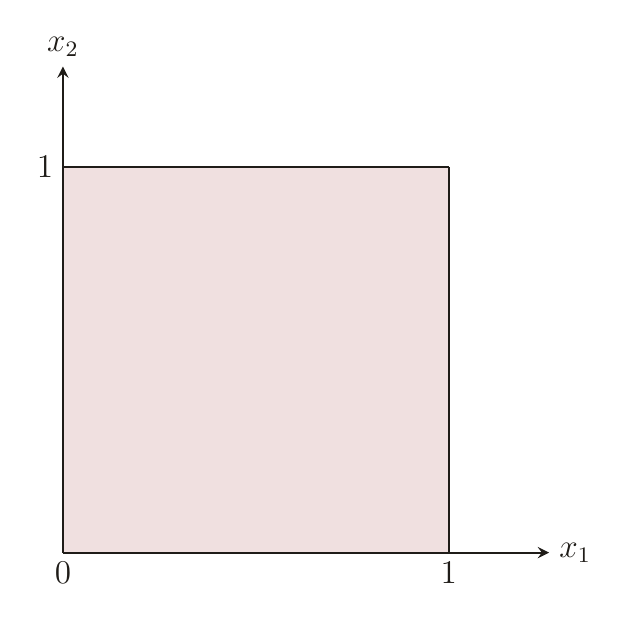
\begin{tikzpicture}[x=4.9cm, y=4.9cm, >=stealth,
                    every node/.style={journalink, font=\large}]

  %% 聯合值域: 單位正方形 0<x_1<1 且 0<x_2<1
  \fill[journalaccent, fill opacity=0.15] (0,0) rectangle (1,1);

  %% 值域的上邊與右邊, 左邊與下邊即為兩條座標軸
  \draw[journalink, line width=0.8pt] (0,1) -- (1,1);
  \draw[journalink, line width=0.8pt] (1,0) -- (1,1);

  %% 座標軸
  \draw[journalink, line width=0.8pt, ->] (0,0) -- (1.26,0) node[right] {$x_1$};
  \draw[journalink, line width=0.8pt, ->] (0,0) -- (0,1.26) node[above] {$x_2$};

  %% 刻度標示
  \node[below] at (1,0) {$1$};
  \node[below] at (0,0) {$0$};
  \node[left]  at (0,1) {$1$};

\end{tikzpicture}
\end{document}
